\chapter{检索增强生成（RAG）}\label{检索增强生成}

\section{检索增强生成 RAG 让回答获得外部依据}\label{检索增强生成 RAG 让回答获得外部依据}

小助能解方程，却不知道``本周作业最晚何时提交''。提交时间由课程最新通知决定，相关材料保存在课程资料库中。我们让小助先检索通知，再根据通知中的日期与适用条件回答。

检索增强生成（Retrieval-Augmented Generation，RAG）已经成为大模型应用中的基础技术，广泛用于企业知识库问答、客服助手、产品文档查询和内部资料检索。它把信息检索与语言生成连接起来：检索系统负责找到当前问题需要的材料，语言模型负责阅读材料并组织回答。资料库可以独立维护，新通知或新文档进入检索范围后，模型就能在回答时使用这些内容。

RAG 的核心是把检索到的外部材料纳入生成条件。模型利用参数中学到的语言与任务能力理解问题，以可更新资料库中的材料作为回答依据。回答质量取决于资料是否准确、检索是否完整，以及模型能否正确解释和引用证据。保存检索结果与来源位置，可以沿这些环节检查答案的形成过程。

\textbf{先区分建库与回答两个阶段}~建库阶段把 PDF、网页或办公文档解析成文本，保留标题、表格和来源信息，再切分、编码并建立索引。扫描版文件可以先通过光学字符识别（Optical Character Recognition，OCR）取得文字。回答阶段接收用户问题，检索相关片段，将片段与问题一起送入模型。常见的工程流程可以复用已有嵌入模型与生成模型，更新资料主要涉及文档处理和索引维护，生成模型的参数保持固定。

我们先把课程文件切成段落。按固定长度切分容易把``允许迟交''和``超过多久不计分''分到两个片段，读者需要结合两个片段才能得到完整规则。我们结合标题、段落、表格与适度重叠，让每个文本片段（chunk）保有必要上下文，同时保存文档名、版本、页码或段落编号。重叠过多会增加重复检索，切得太大又会把相关句子淹没在噪声里，因此要用查询与证据覆盖率选择。

接着，我们用嵌入模型把每个片段编码成向量，并把向量、原文与来源标识关联保存。索引是用于快速找到候选片段的数据结构，可以由向量数据库、搜索引擎或本地检索程序提供。收到问题后，同一个嵌入模型把问题编码成查询向量，检索程序按向量相似度选出候选片段，这个步骤称为召回。常用的余弦相似度衡量两个向量方向的接近程度，得分用于排序候选的相关性。资料量较大时，近似最近邻（Approximate Nearest Neighbor，ANN）索引用较少的比较找到接近查询向量的候选，提高检索速度。若课程名称或作业编号很关键，可以同时做最佳匹配 25（Best Matching 25，BM25）等词法检索，再融合结果。向量检索利用语义联系匹配不同措辞，词法检索利用关键词匹配课程名称、作业编号等精确信息。混合检索将两类候选合并，再通过重排选出与问题最相关的材料。

召回后，我们可用交叉编码器（cross-encoder）重排。双塔嵌入先把查询和文档分别编码，便于大规模比较；cross-encoder 让查询与候选一起进入模型，进行更细的相关性判断，代价也更高。我们因此只用它处理有限候选。

最后，我们把少量证据与问题一起交给小助，要求回答中标明依据，证据不足时说明缺口。检索程序按用户访问权限筛选可用文档，生成器把检索片段作为待分析的资料处理。工具权限与任务规则由应用层管理，文档中的操作性文字按资料内容解释。

\textbf{把一次问答完整走通}~假设课程资料中有三个片段：片段 A 说明作业一的提交时间，片段 B 说明作业二截止于周五 18:00，片段 C 说明迟交扣分规则。用户问``作业二什么时候交？''，系统先检索一批候选，再把最相关的片段 B 放到前面。工程中常把返回得分最高的 $k$ 个候选称为 top-$k$，其中 $k$ 是候选数量；例如先召回 20 个片段，再重排选出 3 个组成模型输入。召回数量决定初选范围，最终选入数量则影响阅读成本与证据覆盖。

交给生成器的输入可以组织成下面的形式：
\begin{quote}
任务：依据课程资料回答问题，给出资料编号。\\
资料 [1]：《课程通知》第 2 节，作业二于周五 18:00 截止。\\
问题：作业二什么时候交？
\end{quote}
模型据此回答``作业二于周五 18:00 截止，依据《课程通知》第 2 节 [1]''。检索阶段选出的文字通过上下文进入这次前向计算，来源标识则把答案与原文位置连接起来。若用户继续询问迟交规则，系统可围绕新问题检索片段 C，再生成对应解释。

资料维护也沿着同一条链进行。课程通知更新时，为新版本重新切分和编码，并更新索引中的对应记录；旧版本可以归档，并用生效日期与版本字段区分。查询时先按课程、年份和访问权限筛选，再在符合条件的资料中检索，回答便能对应到当前适用的通知。

图 \ref{fig:RAG证据链} 将离线建库与在线回答分成两条路径。离线索引保存可检索的表示与来源，在线过程才根据这次问题选择证据。

\begin{figure}[t]
    \centering
    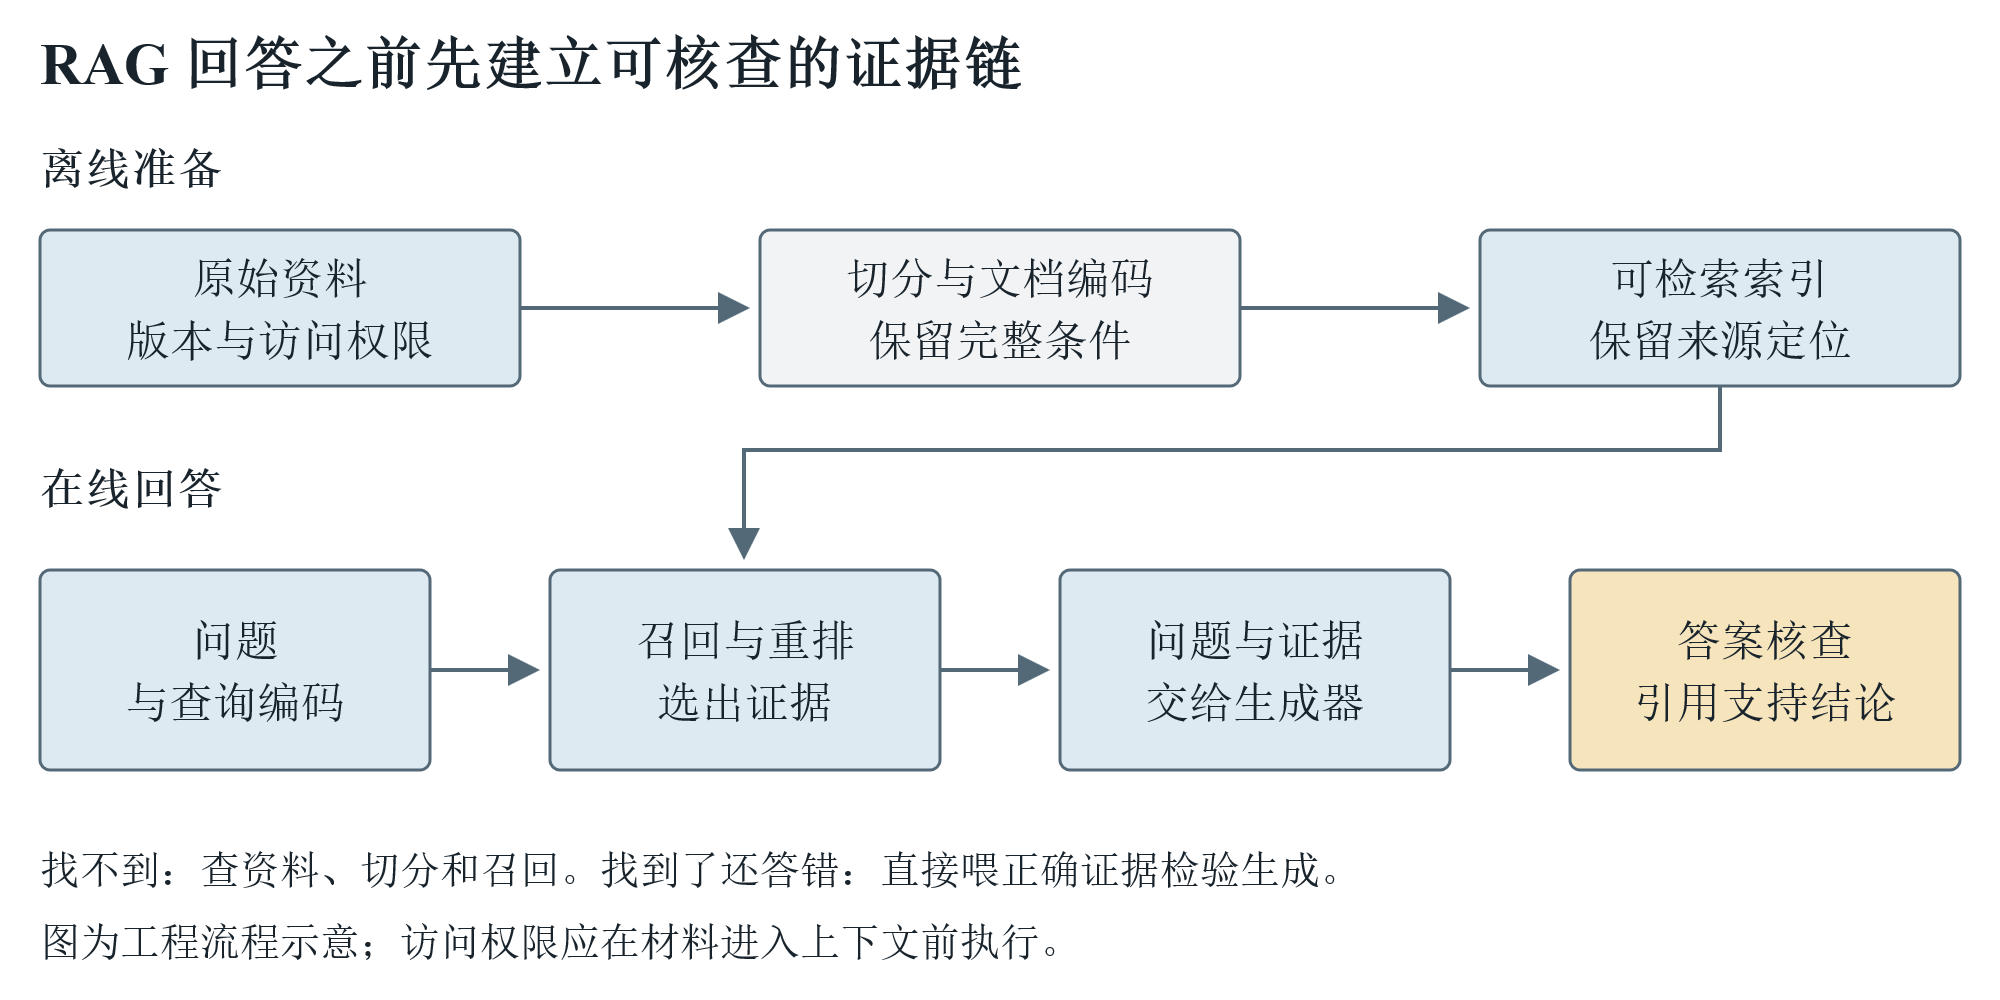
\includegraphics[width=\linewidth]{assets/media/image20.png}
    \caption{RAG 的工程证据链。资料版本、访问权限和来源定位贯穿流程；正确证据交给生成器后是否仍答错，是下一节诊断的关键分叉。}
    \label{fig:RAG证据链}
\end{figure}

我们完成的是一条可逐段检查的证据链：正确材料存在吗，切分保留了吗，召回找到了吗，重排留下了吗，生成忠实使用了吗？下一节就沿这条链定位失败。

\textbf{本节相关资料}
\begin{enumerate}
    \item Lewis 等，2020，\href{https://arxiv.org/abs/2005.11401}{Retrieval-Augmented Generation for Knowledge-Intensive NLP Tasks} 。阅读重点：参数化知识与外部检索如何结合。原论文联合建模检索与生成，工程实践也常采用分别训练的检索器与生成器组成管线。
    \item \href{https://cloud.google.com/use-cases/retrieval-augmented-generation}{Google Cloud：What is Retrieval-Augmented Generation (RAG)?}。阅读重点：RAG 的基本流程与知识库问答等应用场景。
    \item Nogueira 与 Cho，2019，\href{https://arxiv.org/abs/1901.04085}{Passage Re-ranking with BERT} 。阅读重点：联合编码查询与文档为什么适合重排。
\end{enumerate}

\section{RAG 诊断 沿证据链定位失败}\label{RAG 诊断 沿证据链定位失败}

我们问``作业允许迟交几天''，小助引用了一段相关资料，却答错限制条件。只看最终答案，我们不知道该换嵌入模型、扩大上下文，还是重训生成器。我们于是为每个失败保存完整过程：查询、候选、分数、选入上下文的证据和最终回答。

第一步做 oracle context 实验：直接把人工确认的正确证据交给生成器。如果这时仍答错，优先检查阅读、提示、冲突处理或任务能力；如果这时答对，问题更可能在前面的检索与组织。正确证据条件下的回答结果，为后续选择检索侧或生成侧的改进提供依据。

\textbf{用小型评测集建立基线}~可以先收集一组真实问题，为每个问题标出正确答案和支持答案的资料位置。检索阶段检查正确证据是否进入候选，生成阶段检查答案是否正确、引用是否支持结论。若一个问题有 4 个标注为相关的片段，前 $k$ 个检索结果找到了其中 3 个，该问题的召回率 Recall@$k$ 就是 $3/4=75\%$；如果前 $k$ 个结果中有 3 个相关片段，精确率 Precision@$k$ 就是 $3/k$。这里 $k$ 表示检查的检索结果数量。多个问题分别计算后取平均，可以比较切分、检索与重排配置。

对于需要合并多份材料的问题，还要检查关键证据是否收齐。例如，判断某次迟交是否扣分，需要同时取得截止时间与迟交规则。生成侧则逐项核对日期、数值、条件和来源，并记录响应延迟与输入 token 数。证据覆盖、答案质量与运行成本一起构成 RAG 入门系统的评估记录。

随后逐段检查。正确证据不在资料库，是信息缺失；原文有而 chunk 不完整，是切分问题；穷举相似度能找到、ANN 找不到，是索引召回问题；召回中有、重排后丢了，是重排问题；上下文中有、答案仍歪曲，是生成使用问题。每次只替换一个组件，并比较相同查询上的证据与答案变化，就能判断改动影响了哪个环节。

若查询太短或术语错位，可以尝试查询改写。假设文档嵌入（Hypothetical Document Embeddings，HyDE）先生成一个假设性文档，再用它做检索桥梁；假设文档提供与目标材料接近的语义表达，作为检索查询的中间表示；最终回答引用实际检索到的原始资料。

若用户问的是整套课程材料的共同主题，系统需要汇总跨文档信息。图检索增强生成（Graph Retrieval-Augmented Generation，GraphRAG）通过实体、关系或社区摘要组织材料，支持全局主题归纳；建库流程相应增加关系抽取、建图和摘要更新。对于需要逐步补全证据的问题，智能体式检索增强生成（agentic RAG）根据当前结果识别信息缺口，再发起下一次检索。第七章的工具调用循环在这里具体表现为查询、阅读结果、补充查询与组织答案。

对于规模可控、需要跨段联系的资料，可以直接把完整材料放入长上下文，建立综合阅读基线。评估时检查不同证据位置下的回答质量、跨段信息整合能力，以及输入长度带来的延迟和成本。对于持续更新的大型资料库，先检索再阅读可以缩小每次输入的材料范围；检索与长上下文结合，则能把多份相关文档交给模型联合分析。下表按信息获取与行为调整的需求，列出可比较的方案。

\begin{longtable}[]{@{}
  >{\raggedright\arraybackslash}p{(\linewidth - 4\tabcolsep) * \real{0.2985}}
  >{\raggedright\arraybackslash}p{(\linewidth - 4\tabcolsep) * \real{0.2985}}
  >{\raggedright\arraybackslash}p{(\linewidth - 4\tabcolsep) * \real{0.4030}}@{}}
\toprule\noalign{}
\begin{minipage}[b]{\linewidth}\raggedright
\textbf{需求}
\end{minipage} & \begin{minipage}[b]{\linewidth}\raggedright
\textbf{优先建立的基线}
\end{minipage} & \begin{minipage}[b]{\linewidth}\raggedright
\textbf{关键验证}
\end{minipage} \\
\midrule\noalign{}
\endhead
\bottomrule\noalign{}
\endlastfoot
少量完整资料的综合阅读 & 长上下文直接阅读 & 位置变化与跨段整合 \\
经常更新的大型资料库 & RAG & 召回和引用支持度 \\
稳定改变输出行为或格式 & SFT & 新行为与旧能力回归 \\
新知识与新行为同时需要 & 检索与训练组合 & 分别测信息获取和行为执行 \\
\end{longtable}

\textbf{本节相关资料}
\begin{enumerate}
    \item Gao 等，2022，\href{https://arxiv.org/abs/2212.10496}{Precise Zero-Shot Dense Retrieval without Relevance Labels}，HyDE 。阅读重点：假设文档怎样构造检索表示，以及原始资料怎样支持最终回答。
    \item Edge 等，2024，\href{https://arxiv.org/abs/2404.16130}{From Local to Global A Graph RAG Approach to Query-Focused Summarization} 。阅读重点：全局问题与局部段落检索的差别。
    \item Liu 等，2023，\href{https://arxiv.org/abs/2307.03172}{Lost in the Middle How Language Models Use Long Contexts} 。阅读重点：证据位置与输入长度怎样影响模型的信息利用。
\end{enumerate}
